\chapter{Conclusions and Future Work}
\label{chapter:Conclusions}
\thispagestyle{myheadings}
\graphicspath{{6_Conclusion/Figures/}}

% set this to the location of the figures for this chapter. it may
% also want to be ../Figures/2_Body/ or something. make sure that
% it has a trailing directory separator (i.e., '/')!
\graphicspath{{6_Conclusion/Figures/}}
This chapter contains conclusions, discussions and a summery of this dissertation. Part of the discussions will outline future work from the results of the thesis.

This thesis outlined some of the basic theory behind ISR. It then followed with the modeling of the space-time ambiguity function which gives a forward model for ISR systems with electronically scanned arrays. A methodology to simulate complex voltage data for ISR was shown and is available as a software package called SimISR. Lastly using the space-time ambiguity a method to invert ISR data within the frame of reference of moving plasma and improve the resolution of the data has been developed. The inversion method was tested using SimISR in from a set of two-dimensional ionosphere plasma state parameters.

\section{Space-Time Ambiguity Function}
The space-time ambiguity function, discussed detail in Chapter \ref{chapter:stamb}, gives theoretical framework for the optimal analysis of volumetric data acquired from electronically steerable ISR systems. The framework developed here takes into account the full antenna beam pattern, pulse pattern and time integration.

The need for this new framework was shown Section \ref{sec:sptimesamp}, which highlights the sampling paradigm change brought on by ESA systems used in ISR. Due to the ability of ESA systems to have near instantaneous look angle transitions lattice like sampling network develops and decouples space and time sampling for these systems.

The space-time ambiguity is derived in Section \ref{sec:sptimeamb}. This is an extension of the range ambiguity in traditional single beam ISR processing, adding beam pattern and integration time into account. The impact of this ambiguity can be modeled as a Fredholm integral equation of the first kind applied to the ACFs, thus bringing this in line with many similar problems from image formation and processing.

This ambiguity can be extended and augmented to take into a count the inherent motion of the plasma. Section \ref{sec:frametrans} shows how a Galilean Transform can be used to to understand possible motion induced artifacts can be explained. The impact of motion of plasma on the ambiguity was shown through an example beam pattern.

The chapter concluded with an example from the RISR system to show how this could impact data analysis. A possible feature,  much smaller than that shown in the radar reconstruction, was shown to be able to recreate a qualitatively similar formation from the example showed in the data. 
  
\section{SimISR}


The ISR measurement process from an ESA equipped system can be difficult to understand from a purely analytic formulation. Because of this a simulation tool, called SimISR, was developed and discussed in Chapter \ref{chapter:stisrs}. This tool encapsulates the full ISR measurement process, incorporating ESA radar capabilities and the full radar space-time ambiguity along with inherent ISR error sources. 

The methodology for the creation of complex voltage level data can be broken down in to a number of digital signal processing functions. This creates shaped complex Gaussian data using AR filters derived from the ISR spectra, windowed by the pulse shape and summed together within each beam.  

Possible uses for SimISR in the research community have also been discussed and examples have been shown. These examples show how one can use the simulator to create large statistical data sets and also to more optimally design ionospheric radar experiments in the ISR space within the inherently large number of free parameters afforded by the radar control parameters. Researchers can use SimISR to iterate through different set ups for their experiments, as opposed to a heuristic selection of a single observational approach where prior use is the sole design factor. 
 
\section{Inversion of ISR Data}


Finally, using the theoretical and simulation infrastructure developed in the earlier chapters an inversion framework was developed in Chapter \ref{chapter:inversion}. This framework relies on reconstructing the ACFs by finding a regularized solution that has least squares error between it and the data. This has been seen in the past in the image reconstruction literature \citep{Karl:2005jy}.

The process of estimating the ionosphere plasma state parameters by ISR can be represented as a set of linear and non-linear operators. These operations include the non-linear transformation of plasma parameters to and from ACFs and the Space-Time Ambiguity function covered in earlier chapters. In order to use techniques seen in image reconstruction the ACF is descritized along space-time and lag and placed in a single vector. From there the space-time ambiguity function can be represented as a matrix that translates the lags from a Cartesian coordinate space to a radar centered spherical coordinate space. 

The matrix for the forward model can be further augmented to take into account the motion of the plasma. Allowing for the reconstruction the state parameters in the frame of reference of the plasma. This problem holds many similarities for the removal of motion blur in images.

With the problem formulated different constraints are used on the inversion. These constraints include $l^2$-norm constraints on the solution, the derivative of the solution and finally an $l^1$-norm constraint of the derivative. Using a simpler phantom the $l^2$-norm constraint on the derivative has promising results comparatively to the others. This is also holds true for the case using an example set of ionosphere state parameters from \citet{Perry:2015jf} as an input for SimISR. The limit of this study is obvious in that there are a number of different types of distributions that are possible for ionosphere state parameters and that we have looked at a small variety. Also, parametric estimation techniques should be explored to improve the reconstructions. 

\section{Future Research Directions}

There are a number of different areas of research that can be explored from the content of this thesis. Among these are use of simulation tools developed and improvement in the inversion techniques.


\subsection{Further Development of SimISR}

In the future, SimISR development will continue by adding new radar waveform modes, as currently only Barker code and uncoded single pulse modulations are available at this time. The simulator can also be used to create synthetic data for traditional single antenna based system design applications. Other possible expansions of the simulator include capability to calculate returns from each receiver element in a ESA based ISR system, such as the planned architecture of EISCAT-3D, along with multi-static radar capabilities. These future additions will increase the simulator's value to designers who wish to more optimally exploit the capabilities of new systems. 

\subsection{Experiment Planning Using SimISR}

A more immediate application of the SimISR tool can aid researchers in experiment planning. There are a number of phenomena that change on very small spatio-temporal scales, e.g. at high latitudes, and capturing observations of them would greatly benefit from optimization of the experiment set up. 

The ability of SimISR to directly create complex receiver voltage data provides a significant and novel capability, as some geophysical phenomena, such as those that occur at time scales on the order of an IPP, can only be fully explored at this data level. This could lead to researchers coming up with new ways to analyze data, such as novel integration schemes to resolve phenomena at small spatio-temporal scales.

One phenomena that could be better studied using this type of simulation is called pulsating aurora. This flickering of auroral light, along time scales of 5-40 seconds, corresponds to changing ionosphere state parameters caused by precipitating electrons \citep{JGRA:JGRA21510}. The phenomena can take an arc like shape and extend over hundreds of kilometers \citep{JGRA:JGRA20202}. The short modulation period along with the large range extent make this a challenging target to image with an ESA ISR. Researchers can use SimISR to run a number of case studies to determine possible beam and pulse patterns to sample the parameter modulation. Also the researchers can use software developed for SimISR to process the data in different ways such as summing the returns from different beams and range samples together to get a high time cadence to sample the temporal modulation properly. 

Researchers have used ISR as a method to measure electron energy spectra \citep{Semeter:2005foa}. In lower altitudes the electron density measurements can be used the estimate plasma production rates, which can be inverted to show the energy spectra of photons impacting the ionosphere and give remote information about magnetospheric activity. Using SimISR researchers could perform simulations to determine the limits of these techniques and plan experiments where they can be used to great affect.

Multi-sensor campaigns can gain much from capability that SimISR has to assist in planning. Many researchers perform rocket campaigns and use ISR systems to help confirm their measurements \citep{JGRA:JGRA50924}. The same can be said for satellite measurements as well such as the ANDESITE program \citep{parham2016multi}. 

Another exciting development in the geoscience community is future use of the High Frequency Active Auroral Research Program (HAARP) facilities \citep{Bernhardt:2016il} along with a possible co-located AMISR system. Again, SimISR can assist with experiment planning and data analysis from these future experiments.



\subsection{Training Sets for Parameter Fits}

The non-linear inversion step between ACFs and plasma state parameters has a number of built in assumptions, one of the most common is that plasma is Maxwellian distributed. Various physical processes can cause this assumption to be broken which can lead to incorrect parameter fits \citep{St1979ion,Suvanto1988incoherent,Akbari:2015fv}. Events that cause this can be hard to find so machine learning techniques could be useful in finding these events ISR databases \citep{Duda:2000:PC:954544}. Many of these algorithms require training data sets, which to could be a labor intensive and tedious task. SimISR could be used to make these sets and they could feed into different pattern matching algorithms and help catalog incorrectly fitted data.

\subsection{Inversion Techniques}

There are a number of different improvements that can be done for the inversion methods highlighted in this thesis. Currently the techniques have only been applied to two dimensional distributions of plasma state parameters. Extention to three dimensional distributions may require more software development to be allowed to run on graphics processor units which can perform large numbers of parallel processes. The inversion techniques could also be applied to real ISR data using techniques outlined in \citet{butler:imagingfregiondrifts} to first estimate the parameter drifts and then invert within the frame of reference of the motion.

Estimation of the ACFs could also be improved by investigating the literature studying time-varying channels and overspread targets \citep{Kailath:1962jx,Kailath:1963gh,Pfander:2006hh,Pfander:2015ea}. A deeper investigation of this can yield a better understanding of the processing and its limitations using time-frequency analysis \citep{TFAcohen,Peyrin:1986bh,Jiang:kj}. From a practical point of view there have already been a number of algorithms that have already been proposed to estimate ACFs from overspread targets \citep{Pfander:2015ea,Jiang:kj}. One example seen in \citet{Kay:2003jl} can yield an estimation algorithms similar to those seen in synthetic aperture radar and modalities that use similar models to invert a scattering field \citep{1456966,Ralston:2007hs,richards2014fundamentals}. Another aspect of this that could be investigated is the use of spherical harmonics for different interpolation schemes \citep{Baddour:2010cq,Baddour:2009jm,Baddour:2012bd}.

Parametric techniques for inverting directly to plasma state parameters need to be investigated. There are a number of different schemes including those that use dynamic programing that could be useful \citep{Yau:1992kd,Yau:1993kf,Oktem:2014ju}. New algorithms for parameter fitting also need to be investigated and incorporated as well \citep{Shpynev:2010co}. This could be used to extend \textit{Full Profile Analysis}, seen in \citet{RDS:RDS3308,hysell2008}, to, what can be called \textit{Full Volume Analysis} to measure plasma parameters.

\subsection{Sensor Data Fusion}

Other types of sensors can be useful to understand the ionosphere, be it optical sensors such as all sky imagers to GPS TEC measurements. Even combining satellite magnetometer data from the AMPERE project \citep{Anderson:2000uh,Anderson:2014hf}, along with green line emission all sky data a number of interesting things can be learned. If Figure \ref{fig:swflow} incredibly structured magnetic field deflections at the time of a large increase in auroral emissions. This can give a large amount  information as to the state of energy flux within magnetosphere and ionosphere

\begin{figure}[h!]
\centering
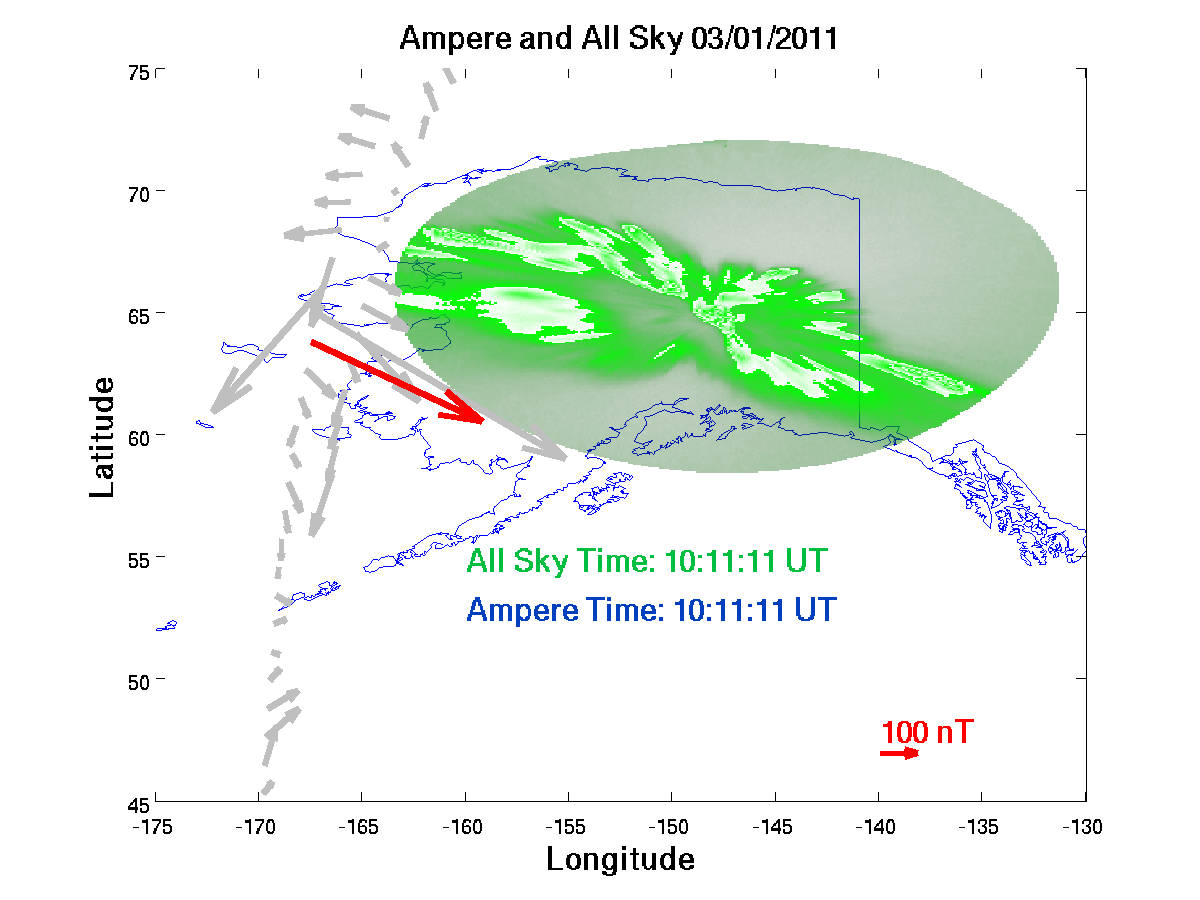
\includegraphics[width=6.0in]{ampandallsky214}
\caption{Combination of AMPERE magnetic deflection data and All Sky green line emissions. }
\label{fig:swflow}
\end{figure}

This sort of sensor fusion experiments can be very useful but can also be time consuming. In order to help speed along the process of analysis a software package, called \textit{GeoData} was developed. It is available in both the MATLAB \citep{john_swoboda_2016_154536} 
and Python \citep{john_swoboda_2016_154533} programing languages. This software package abstracts each data set into a standard object format to increase the reusability of code across different research tasks. This package was built to allow for data from multiple sensors to be quickly registered, analyzed and plotted. This type of advanced programing interface (API) allows for greater software reuse by abstracting sensor data to common format. GeoData and other pieces of software are described in more detail in Appendix \ref{chapter:appsoft}.

Sensor fusion techniques can go a step further and be directly involved in the reconstruction of plasma parameters such as shown in \citet{Semeter:2016gm}. For example, information added by the GPS TEC measurements can be incorporated in algorithms that use the Space-Time Ambiguity formulation. This could help improve reconstruction of all of the ISR systems plasma state parameters if implemented properly.
